% Created 2021-01-24 Sun 22:49
% Intended LaTeX compiler: pdflatex
\documentclass[11pt]{article}
\usepackage[utf8]{inputenc}
\usepackage[T1]{fontenc}
\usepackage{graphicx}
\usepackage{grffile}
\usepackage{longtable}
\usepackage{wrapfig}
\usepackage{rotating}
\usepackage[normalem]{ulem}
\usepackage{amsmath}
\usepackage{textcomp}
\usepackage{amssymb}
\usepackage{capt-of}
\usepackage{hyperref}
\usepackage{minted}
\hypersetup{colorlinks=true, linkcolor=black, filecolor=red, urlcolor=blue}
\usepackage[turkish]{babel}
\author{Eren Hatırnaz}
\date{29 Mart 2020}
\title{Yazılım Gündemi - 2020/12\\\medskip
\large 23-29 Mart 2020}
\hypersetup{
 pdfauthor={Eren Hatırnaz},
 pdftitle={Yazılım Gündemi - 2020/12},
 pdfkeywords={},
 pdfsubject={},
 pdfcreator={Emacs 27.1 (Org mode 9.3)},
 pdflang={Turkish}}
\begin{document}

\maketitle
\tableofcontents \clearpage\shorthandoff{=}

\begin{center}
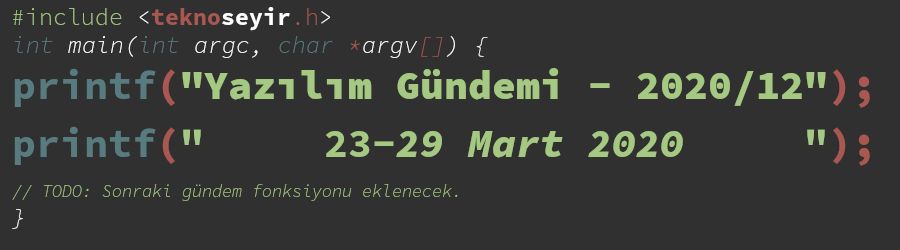
\includegraphics[width=.9\linewidth]{gorseller/yazilim-gundemi-banner.png}
\end{center}

\begin{center}
\href{../11/yazilim-gundemi-2020-11.pdf}{< Önceki Gündem} | \textbf{23-29 Mart 2020} | \href{../13/yazilim-gundemi-2020-13.pdf}{Sonraki Gündem >}

\href{https://teknoseyir.com/blog/yazilim-gundemi-2020-12}{TeknoSeyir'de Oku}
\end{center}

\section{Safari 13.1 ile tüm üçüncü parti \href{https://www.engadget.com/2020-03-24-safari-blocks-all-third-party-cookies-by-default.html}{çerezleri engellemeye başladı}}
\label{sec:orgab5f824}
Bu hafta içerisinde yayınlanan iOS ve iPadOS güncellemeleri ile birlikte Apple
ekosisteminin varsayılan tarayıcısı olan Safari, artık tüm üçüncü parti
çerezleri (cookie) engelliyor. Intelligent Tracking Preventation (ITP) isimli
özelliklerindeki bu güncellemenin amacı ise kullanıcıların internette
gezinirken takip edilmesini önlemek. Bu derece sert bir kuralı uygulayan bir
diğer tarayıcı ise Tor Browser. Brave Browser ise bazı istisnalar hariç diğer
çerezleri engelliyor.

İlgili değişiklikler Apple tarafından açık kaynak olarak geliştirilen tarayıcı
motoru WebKit'in \href{https://webkit.org/blog/10218/full-third-party-cookie-blocking-and-more/}{blog sayfasında duyuruldu}. Yazıda bu yolda yalnız
olmadıklarını Google tarafından geliştirilen Chrome tarayıcısının da 2022 yılı
için bu tarz bir \href{https://blog.chromium.org/2020/01/building-more-private-web-path-towards.html}{değişikliğe hazırlandığını} belirtmiş. Aynı zamanda bu
uygulamanın standart olması için W3C kurumuna da başvuracaklarını
belirtmişler.

Değişikliğin biz geliştiricileri etkileyen kısmında ise bizlere üçüncü parti
çerezler yerine kullanabileceğimiz 3 farklı opsiyon sunmuşlar. Bunlar şu
şekilde:

\begin{itemize}
\item \href{https://tools.ietf.org/html/rfc6749}{OAuth 2.0 Authorization}
\item \href{https://webkit.org/blog/8124/introducing-storage-access-api/}{The Storage Access API}
\item Popup'lar için \href{https://webkit.org/blog/8311/intelligent-tracking-prevention-2-0/}{Geçici Uyumluluk Çözümü}
\end{itemize}

Fakat bu değişiklikler sadece çerezleri etkilemiyor. Tarayıcıda bazı verileri
depolamak için kullandığımız IndexedDB, LocalStorage ve SessionStorage gibi
yapılar da etkileniyor. Artık bu yapılar üzerinde sadece 7 günlük veriler
tutabileceğiz. Bunu yapmalarındaki amaç ise büyük ihtimal kullanıcıları takip
eden servislerin çerez engellemesini bu tarz yapıları kullanarak aşmalarını
istememeleri olabilir.

Bu konu hakkında siz ne düşünüyorsunuz? Safari'nin çerezlere olan bu sert
yaklaşımı siz doğru mu? Yorumlar bölümünde konuşalım.
\section{Git 2.26 \href{https://lore.kernel.org/git/xmqqa7477u6j.fsf@gitster.c.googlers.com/T/\#u}{sürümü yayınlandı}}
\label{sec:org3dcbe6b}
En popüler versiyon kontrol sistemlerinden biri olan Git, bu hafta içerisinde
2.26 numaralı yeni sürümünü duyurdu. Bu sürüm ile birlikte gelen bazı
değişikliklere birlikte bakalım.

\subsection{Varsayılan protokol versiyonu 2 olarak güncellendi}
\label{sec:org5510638}
2018 yılında Git'e Google tarafından katkı sağlanarak eklenen \emph{Git protocol
version 2} artık varsayılan olarak kullanılacak. Önceki Git protokolünün bazı
ölçekleme sorunları vardı. Bir Git sunucusu, istemci (client) özel olarak
istemediği halde tüm branch'lar, tag'lar ve diğer referanslar hakkında bilgi
veriyordu. İlk bakışta "bunda ne var" diye düşünebilirsiniz ama büyük çaplı
projeler için durum böyle değil. Kullanıcı sadece master dalıyla ilgilendiği
halde ona tüm dallar ve etiketlerle ilgili bilgi dönmesi demek fazladan
birkaç megabyte'ın harcanması demek ve bu da gereksiz veri trafiği anlımına
geliyor. Şimdi ise büyük boyutlu depolardan daha kısa bir sürede veri
çekebiliyor olacağız.

Eğer Git versiyonunuzu yükseltmeye henüz hazır değilseniz ve Git 2.19 üzeri
bir sürüm numarasına sahipseniz. Bu değişikliği siz de aşağıdaki komutu
çalıştırarak uygulayabilirsiniz:

\begin{minted}[breaklines=true,breakanywhere=true]{shell}
git config --global protocol.version 2
\end{minted}

Bu protokol versiyonu hakkında daha detaylı bilgi almak için \href{https://opensource.googleblog.com/2018/05/introducing-git-protocol-version-2.html}{bu sayfayı
ziyaret edebilirsiniz}.
\subsection{\texttt{git sparse-checkout} komutunda değişiklikler}
\label{sec:orgbd32d74}
Bir önceki sürüm (2.25) güncellemesiyle birlikte gelen bu özelliği \href{../03/yazilim-gundemi-2020-03.pdf}{Yazılım
Gündemi - 2020/03} yazısında detaylıca anlatmıştık. Dolayısıyla özelliğin
teknik detayları için önce o yazıyı okumanızı tavsiye ederim. Bu sürümle
ise \texttt{git sparse-checkout add} modu eklendi. Artık daha kolay bir şekilde
istediğimiz klasörleri indirebileceğiz. Örnek kullanım için:

\begin{verbatim}
$ git clone --filter=blob:none --sparse git@github.com:git/git.git
$ cd git
$ git sparse-checkout init --cone
$ git sparse-checkout add t
$ git sparse-checkout add Documentation
$ git sparse-checkout list
Documentation
t
\end{verbatim}
Yukarıda sırasıyla şu işlemleri yaptık:
\begin{enumerate}
\item github.com/git/git deposunu sparse-checkout özelliğini kullanarak clone
edeceğimizi belirttik.
\item \texttt{git} klasörünün içine girdik. sparse-checkout yapacağımız için içi boş.
\item \texttt{sparse-checkout} özelliğini başlattık.
\item \texttt{t} isimli klasörü uzak sunucudan indirdik.
\item \texttt{Documentation} isimli klasörü uzak sunucudan indirdik.
\item \texttt{sparse-checkout} yaptığımız klasörlerin listesini yazdırdık.
\end{enumerate}

Git 2.26 sürümüyle birlikte gelen diğer yeni özellik ve değişiklikler için
GitHub tarafından hazırlanmış \href{https://github.blog/2020-03-22-highlights-from-git-2-26/}{şu blog yazısını okuyabilir} ya da konu başlığına
eklediğim bağlantıya tıklayabilirsiniz.
\section{TypeScript 3.9 Beta \href{https://devblogs.microsoft.com/typescript/announcing-typescript-3-9-beta/}{duyuruldu}}
\label{sec:org01b7531}
Microsoft tarafından geliştirilen JavaScript üreten programlama dili
TypeScript'in bu hafta içerisinde 3.9 Beta etiketli sürümü duyuruldu.
Microsoft TypeScript takımının bloglarında yayınladıkları yazıyı inceledim
fakat dile uzak birisi olduğum için pek bir şey anladığım söylenemez. Bu
nedenle bu sefer de sizi konu başlığına eklediğim bağlantıya tıklayamaya davet
ediyorum. TypeScript'i ilgi alanıma girerse, ilerleyen Yazılım Gündemi
yazılarında daha detaylı değinebilirim belki.

Henüz "Beta" sürecinde olduğu için çalışan projelerinizi bu sürüme geçirmeniz
tavsiye edilmez ama yine de ayrı olarak bir deneme yapmak isterseniz şu komutu
çalıştırarak TypeScript 3.9 Beta'yı projenize ekleyebilirsiniz:
\begin{minted}[breaklines=true,breakanywhere=true]{shell}
npm install typescript@beta
\end{minted}
\section{Google Play üzerindeki Multiplayer API \href{https://support.google.com/googleplay/android-developer/answer/9469745?hl=en}{desteği sonlanıyor}}
\label{sec:org5eb6354}
Gün geçmiyor ki bir başka Google hizmeti ya da ürünü \href{https://killedbygoogle.com/}{Google Mezarlığı}nda
yerini almasın. Android için oyun geliştirirken Google'ın geliştiriciler için
sunduğu oyununuza çok-oyuncu (multiplayer) API desteğini kullanabiliyordunuz.
Google Play üzerinden sağlanan bu API ile birlikte arka plandaki bazı iş
yüklerinden kurtuluyordunuz fakat 31 Mart itibariyle bu özellik artık
çalışmayacak. Eğer sizin de Google Play markette yayınlanmış ve Multiplayer
API kullanan bir oyununuz varsa bu tarihten itibaren çalışmamaya başlayabilir.

Neyse ki bazen Google bir taraftan alırken bir taraftan da yeni alternatifler
koyabiliyor. Bu hafta içerisinde Google Cloud tarafında oyun yönetimi için
\href{https://cloud.google.com/blog/products/gaming/introducing-google-cloud-game-servers}{yeni bir çözüm tanıtıldı}: \href{https://cloud.google.com/game-servers}{Game Servers}. Henüz "beta" etiketiyle sunuluyor
fakat önümüzdeki dönemlerde stabil bir sürüme de kavuşacaktır.
\section{GitHub Desktop uygulamasının 2.4 \href{https://github.blog/2020-03-25-github-desktop-2-4-introduces-proxy-support-and-issue-creation/}{sürümü yayınlandı}}
\label{sec:org3ded677}
\begin{center}
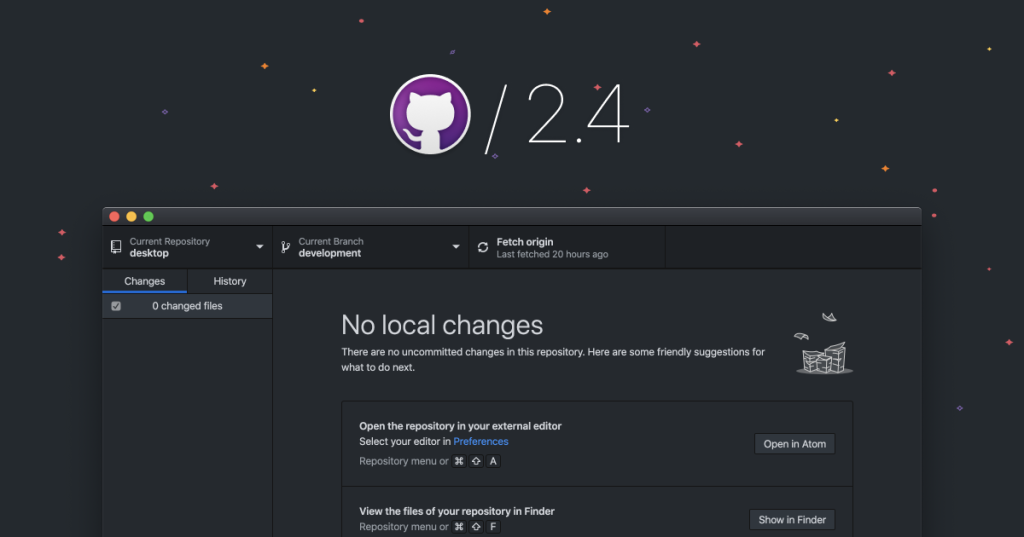
\includegraphics[height=5cm]{gorseller/github-desktop-2.4.png}
\end{center}

GitHub'ın henüz sadece Windows ve Mac işletim sistemlerini destekleyen
masaüstü yazılımı 2.4 sürümüne ulaştı. Bu sürümle birlikte eklenen bazı
özellikler şu şekilde:

\begin{itemize}
\item \textbf{Proxy desteği}: Artık GitHub Desktop uygulamasının internetle olan
bağlantısını bir proxy üzerinden geçirip kullanabileceğiz.
\item \textbf{Issue oluşturmak için kısayol}: Repository menüsü altına "Create Issue on
GitHub" seçeneği eklendi ve tıkladığınızda varsayılan tarayıcınız üzerinde
ilgili deponun issue oluşturma sayfasını açıyor.
\item \textbf{Koyu tema özelliği betadan çıktı}: Çeşitli testler ve geri dönüşlerden
sonra iyileştirilen uygulamanın koyu tema modu sonunda beta'dan çıktı ve
herkese açıldı. Keşke GitHub'ın web arayüzüne de gelse koyu tema özelliği
ya da bu uygulamanın GNU/Linux dağıtımları için olan sürümünü çıkarsınlar o
da uyar bana, gece karanlıkta çalışırken GitHub'ı açınca far görmüş tavşan
gibi kalmaktan bıktım! Zaten olmaması ayrı bir saçmalık. Çoğunlukla
geliştiricilerin kullandığı bir web sitesinde neden koyu tema özelliği
olmaz gerçekten anlamak çok güç.
\end{itemize}

Uygulamayı \href{https://desktop.github.com/}{bu adres üzerinden indirebilirsiniz}.
\section{Diğer Haberler}
\label{sec:orgbf9b730}
\begin{itemize}
\item GitHub, COVID-19 salgınıyla ilgili proje geliştirmek isteyen geliştiriciler
için rehber niteliğinde \href{https://github.blog/2020-03-23-open-collaboration-on-covid-19/}{bir blog yazısı yayınladı}.
\item GitHub Şubat ayı sonlarında yaşanan kesintilerle ilgili \href{https://github.blog/2020-03-26-february-service-disruptions-post-incident-analysis/}{analiz yayınlandı}.
\item GitLab, IPv6 \href{https://gitlab.com/gitlab-com/gl-infra/infrastructure/-/issues/645\#note\_313218618}{desteğini tamamlandı}.
\item Spotify, \href{https://developer.spotify.com/community/news/2020/03/20/introducing-podcasts-api/}{yeni Podcast API'sini duyurdu}.
\item .NET Core Mart Güncellemeleri yayınlandı:
\begin{itemize}
\item \href{https://github.com/dotnet/core/blob/master/release-notes/3.1/3.1.3/3.1.3.md}{.NET Core 3.1.3}
\item \href{https://github.com/dotnet/core/blob/master/release-notes/2.1/2.1.17/2.1.17.md}{.NET Core 2.1.17}
\end{itemize}
\item Microsoft Visual C/C++ için uyumlu preprocessor \href{https://devblogs.microsoft.com/cppblog/announcing-full-support-for-a-c-c-conformant-preprocessor-in-msvc/}{desteği duyuruldu}.
\item COVID-19 Global Hackathon 1.0 \href{https://covid-global-hackathon.devpost.com/}{için kayıtlar başladı}.
\item LLVM 10.0.0 \href{http://lists.llvm.org/pipermail/llvm-announce/2020-March/000087.html}{yayınlandı}.
\item Swift programlama dilinin 5.2 \href{https://swift.org/blog/swift-5-2-released/}{sürümü yayınlandı}.
\item Liberica JDK 14 \href{https://bell-sw.com/announcements/2020/03/18/Liberica-JDK-14/}{sürümü yayınlandı}.
\item Kubernetes 1.18 \href{https://kubernetes.io/blog/2020/03/25/kubernetes-1-18-release-announcement/}{sürümü yayınlandı}.
\item Angular kütüphanesinin 9.1.0 \href{https://github.com/angular/angular/releases/tag/9.1.0}{sürümü yayınlandı}.
\item Kafka-on-Pulsar projesi \href{https://streamnative.io/blog/tech/2020-03-24-bring-native-kafka-protocol-support-to-apache-pulsar/}{duyuruldu}. \href{https://github.com/streamnative/kop}{GitHub Deposu}
\item Cloud için güvenlik aracı Panther \href{https://blog.runpanther.io/panther-v1-open-source-siem/}{açık kaynak olarak tanıtıldı}. \href{https://github.com/panther-labs/panther}{GitHub
Deposu}
\item GraphQL için güvenlik testi araco InQL Scanner \href{https://blog.doyensec.com/2020/03/26/graphql-scanner.html}{açık kaynak olarak tanıtıldı}.
\href{https://github.com/doyensec/inql}{GitHub Deposu}
\item OpenAPIGenerator 4.3.0 \href{https://github.com/OpenAPITools/openapi-generator/releases/tag/v4.3.0}{sürümü yayınlandı}.
\end{itemize}
\section{Lisans}
\label{sec:orga6e56b0}
\begin{center}
\begin{center}

\includegraphics[height=1.5cm]{../../../img/CC_BY-NC-SA_4.0.png}
\end{center}

\href{yazilim-gundemi-2020-12.pdf}{Yazılım Gündemi - 2020/12} yazısı \href{https://erenhatirnaz.github.io}{Eren Hatırnaz} tarafından \href{http://creativecommons.org/licenses/by-nc-sa/4.0/}{Creative Commons
Atıf-GayriTicari-AynıLisanslaPaylaş 4.0 Uluslararası Lisansı} (CC BY-NC-SA 4.0)
ile lisanslanmıştır.
\end{center}
\end{document}
